% !TEX encoding = UTF-8
% !TEX TS-program = pdflatex
% !TEX root = ../tesi.tex

%**************************************************************
\chapter{Descrizione dello stage}
\label{cap:descrizione-stage}
%**************************************************************

\intro{In questo capitolo descriveremo gli obiettivi e il lavoro effettuato nello stage a grandi linee, per poi approfondire nel dettaglio nei prossimi capitoli}\\

%**************************************************************
\section{Introduzione al progetto}
\begin{figure}[!h] 
	\centering 
	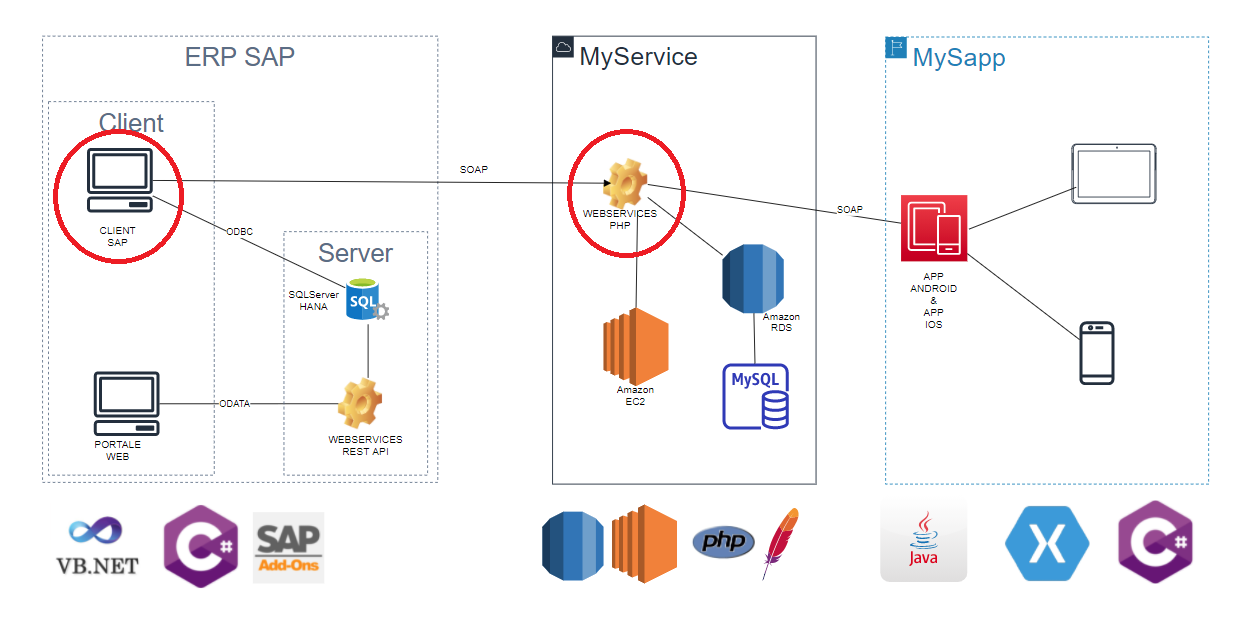
\includegraphics[scale = 0.5]{immagini/obiettivi-stage.png} 
	\caption{Schema infrastruttura preesistente, con evidenziati le componenti obiettivo del lavoro di stage}
	\label{fig:3-1}
\end{figure}
\newpage

	In figura \ref{fig:3-1} possiamo vedere lo schema dell'infrastruttura preesistente, già vista nel capitolo precedente.\\
	Evidenziate in rosso, con un cerchio, possiamo vedere le due componenti su cui è stato concentrato il lavoro durante questo stage:


\begin{itemize}
	\item \textbf{Client SAP:} è stato creato un nuovo add-on, utilizzabile dal client SAP;
	\item \textbf{Webservices PHP:} sono state modificate ed ampliate alcune funzioni che compongono i webservices in PHP.
\end{itemize}
\subsection{Vincoli tecnologici}
L'azienda ha posto due vincoli tecnologici:
\begin{itemize}
	\item nello sviluppo dell'add-on, utilizzare VB.NET oppure C\#;
	\item negli ampliamenti dei webservices solamente il linguaggio PHP.
\end{itemize}
Il vincolo sugli add-on è tale, poichè quest'ultimi possono essere programmati soltanto in quei due linguaggi.

Il vincolo sugli ampliamenti dei webservices è dettato dal dover modificare delle funzioni in PHP, dunque bisogna utilizzare lo stesso linguaggio.
\section{Interazione}
Per lo svolgimento dell'attività di stage si è deciso in comune accordo con il tutor aziendale di svolgere lo stage completamente in azienda.\\
Questo è stato deciso per favorire il dialogo tra studente e tutor aziendale, ed eventualmente un confronto con gli altri dipendenti dell'azienda, esperti nel settore d'interesse.
\section{Requisiti e obiettivi}
Sin dal piano di lavoro sono stati decisi alcuni obiettivi, di cui 3 obbligatori e 1 desiderabile.
\\Obiettivi obbligatori:
\begin{itemize}
	\item Comprensione e apprendimento di strumenti di programmazione e infrastruttura esistente;
	\item Sviluppo protocolli di comunicazione tra i diversi moduli;
	\item Sviluppo applicazione add-on.
\end{itemize}
Obiettivo desiderabile:
\begin{itemize}
	\item Test e documentazione.
\end{itemize}
\subsection{Raggiungimento obiettivi}
Gli obiettivi e risultati raggiunti dall'applicazione sono stati considerati più che sufficienti dall'azienda.
In particolare sono stati raggiunti tutti gli obiettivi obbligatori concordati nel piano di lavoro.

Purtroppo non è stato possibile effettuare test automatici del codice, poichè il codice non è abbastanza corposo da renderli necessari.

%**************************************************************
\section{Pianificazione}
La durata dello stage è stimata attorno alle 320 ore circa.\\
Per ottenere una buona organizzazione dell'attività di stage, è stato stilato il piano di lavoro assieme al tutor aziendale Massimo Ennio e al relatore Massimiliano De Leoni.
\subsection{Piano di Lavoro}
La ripartizione delle ore è stata distribuita nelle 8 settimane in questo modo:
\begin{figure}[!h] 
	\centering 
	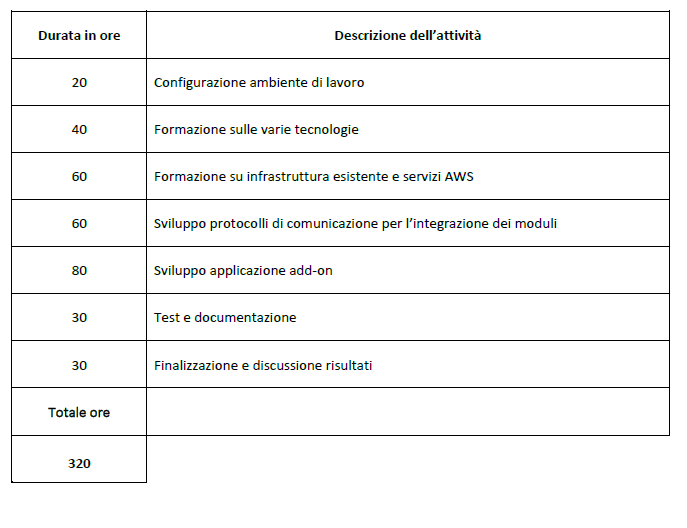
\includegraphics[scale = 0.8]{immagini/ripartizione-ore-piano.png} 
	\caption{Ripartizione ore, secondo il piano di lavoro, durante l'attività di stage}
\end{figure}

